\documentclass{article}
\RequirePackage[numbers,sort&compress,square,comma]{natbib}
\usepackage{graphicx}
\usepackage[a4paper, total={6in, 8in}]{geometry}
\bibliographystyle{IEEEtranN}
\begin{document}
\title{Machine Learning and Applications (MLAP) Open Assessment}
\author{Exam Number: Y0070813}
\date{\vspace{-5ex}}
\maketitle
%\tableofcontents
\section{Task 1}
Code is given in \textit{code/task1/openAssessment.m} and can be executed by running the following command from the task1 directory: \\
\textbf{matlab -nosplash -nodesktop -nofigurewindow -r "openAssessment('\$network.csv','\$data.csv')"}\\


The E-step generates data which is most likely, given the current parameters. Each data-point is split into a set of permutations, one for every combination of the hidden variables. The Bayesian likelihood for each permutation is calculated, to be used as an increment weight in the M-step, effectively calculating the expected value for each hidden variable.

In the M-Step, where new parameters are generated using this imputed dataset, we count the number of times each variable is 1 given each of its parent states and the number of times the parent state occurs, dividing these through to calculate the probabilities to be used in the next E-step. The weights generated in the E step is the increment amount for each count. 

To generate the log-likelihood I sum the log-likelihoods for each data-point, which is calculated by summing the likelihood for each permutation of the data-point's hidden variables, which is itself a product of the probability of each variable.

To detect the convergence of the algorithm I store the Log-likelihood for the previous iteration and compare it to the value calculated on the current iteration, if the difference is greater than 0.0001 then I report convergence.
\newpage
\section{Task 2}
The adaptation of the code was achieved by allowing a file to be given to the main function which specifies each individual starting conditional probability. The adapted code is given in \textit{code/task2/openAssessment.m} and can be executed by running the following command from the task2 directory:\\
\textbf{matlab -nosplash -nodesktop -nofigurewindow -r "openAssessment('\$network.csv','\$data.csv', '\$initialValues.csv')"} \\\\

The EM algorithm finds the local maximum for the Maximum Likelihood Estimator, therefore if there is a multi-modal distribution it is possible that the EM algorithm will not find the global maximum and instead one of many possible local maximums. Additionally, in the case of Bayesian Networks where the posterior probability is calculated from a combination of a prior distribution and a series of observations, if we ensure that there are no observations for a variable its posterior distribution will be based entirely on the prior distribution. To demonstrate this I have used the printer nightmare network again but by removing the observations for variable 1 and 3 I ensure that the posterior distribution, and therefore the parameters chosen by the EM algorithm, are only influenced by the prior distribution, in this case the initial values for the conditional probability. The network topography and dataset used are given in \textit{data/bnprinterTask2.csv} and \textit{bnprinterdataTask2.csv} respectively with initial values for the probabilities given in \textit{data/initialValues.csv}.

Although the adapted code can take individual starting probabilities for each variable, using single values across all variables also demonstrates this. 0.3 and 0.7 are chosen as these two initial values cause their variables parameter to be the initial value, and also have effect on child variables. This is shown in the table below. Additionally a plot of the log-likelihood against the EM iteration number is shown for both initial values.

\begin{center}
\begin{tabular}{|p{7cm}|p{7cm}|}
	\hline
	\begin{center}
		\textbf{Initial Probabilities of 0.3}
	\end{center}
	& 
	\begin{center}
		\textbf{Initial Probabilities of 0.7}
	\end{center}
	\\
	\hline
	\begin{verbatim}
	Convergence in 146 steps 
	Variable 0 has these parents ()
	P(0=1|() = 2.509891e-01 
	
	Variable 1 has these parents ()
	P(1=1|() = 3.000000e-01 
	
	Variable 2 has these parents ()
	P(2=1|() = 4.059554e-01 
	
	Variable 3 has these parents ()
	P(3=1|() = 3.000000e-01 
	
	Variable 4 has these parents ()
	P(4=1|() = 3.159885e-01 
	
	Variable 5 has these parents (0)
	P(5=1|('0')) = 0 
	P(5=1|('1')) = 9.828874e-01 
	
	Variable 6 has these parents (1, 2, 3)
	P(6=1|('0', '0', '0')) = 3.166248e-01 
	P(6=1|('0', '0', '1')) = 3.166248e-01 
	P(6=1|('0', '1', '0')) = 1.000000e+00 
	P(6=1|('0', '1', '1')) = 1.000000e+00 
	P(6=1|('1', '0', '0')) = 3.166248e-01 
	P(6=1|('1', '0', '1')) = 3.166248e-01 
	P(6=1|('1', '1', '0')) = 1.000000e+00 
	P(6=1|('1', '1', '1')) = 1.000000e+00 
	
	Variable 7 has these parents (0, 3)
	P(7=1|('0', '0')) = 2.754369e-01 
	P(7=1|('0', '1')) = 2.754369e-01 
	P(7=1|('1', '0')) = 6.529709e-01 
	P(7=1|('1', '1')) = 6.529709e-01 
	
	Variable 8 has these parents (3, 4)
	P(8=1|('0', '0')) = 1.862551e-01 
	P(8=1|('0', '1')) = 6.273635e-01 
	P(8=1|('1', '0')) = 1.862551e-01 
	P(8=1|('1', '1')) = 6.273635e-01 
	
	Variable 9 has these parents (0, 4)
	P(9=1|('0', '0')) = 4.993921e-01 
	P(9=1|('0', '1')) = 1 
	P(9=1|('1', '0')) = 3.910056e-01 
	P(9=1|('1', '1')) = 9.993642e-01\end{verbatim} & \begin{verbatim}
	Convergence in 64 steps 
	Variable 0 has these parents ()
	P(0=1|() = 4.393333e-01 
	
	Variable 1 has these parents ()
	P(1=1|() = 7.000000e-01 
	
	Variable 2 has these parents ()
	P(2=1|() = 4.059554e-01 
	
	Variable 3 has these parents ()
	P(3=1|() = 7.000000e-01 
	
	Variable 4 has these parents ()
	P(4=1|() = 3.058343e-01 
	
	Variable 5 has these parents (0)
	P(5=1|('0')) = 0 
	P(5=1|('1')) = 4.574197e-01 
	
	Variable 6 has these parents (1, 2, 3)
	P(6=1|('0', '0', '0')) = 3.166248e-01 
	P(6=1|('0', '0', '1')) = 3.166248e-01 
	P(6=1|('0', '1', '0')) = 1.000000e+00 
	P(6=1|('0', '1', '1')) = 1.000000e+00 
	P(6=1|('1', '0', '0')) = 3.166248e-01 
	P(6=1|('1', '0', '1')) = 3.166248e-01 
	P(6=1|('1', '1', '0')) = 1.000000e+00 
	P(6=1|('1', '1', '1')) = 1.000000e+00 
	
	Variable 7 has these parents (0, 3)
	P(7=1|('0', '0')) = 1.259833e-03 
	P(7=1|('0', '1')) = 1.259833e-03 
	P(7=1|('1', '0')) = 7.933800e-01 
	P(7=1|('1', '1')) = 7.933800e-01 
	
	Variable 8 has these parents (3, 4)
	P(8=1|('0', '0')) = 1.962714e-01 
	P(8=1|('0', '1')) = 6.262406e-01 
	P(8=1|('1', '0')) = 1.962714e-01 
	P(8=1|('1', '1')) = 6.262406e-01 
	
	Variable 9 has these parents (0, 4)
	P(9=1|('0', '0')) = 3.596072e-01 
	P(9=1|('0', '1')) = 1 
	P(9=1|('1', '0')) = 6.581454e-01 
	P(9=1|('1', '1')) = 1.000000e+00 
	\end{verbatim}\\ 
	\hline
\end{tabular} 
\end{center}

\begin{figure}[h!]
\centering
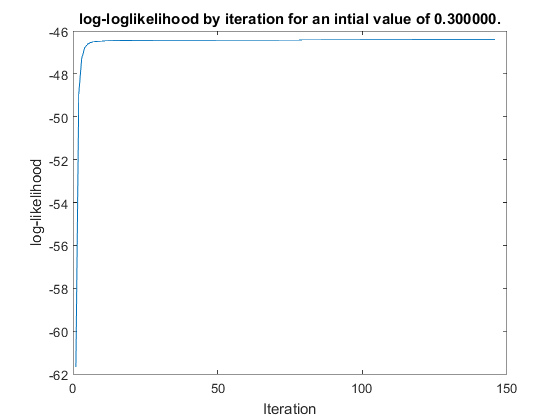
\includegraphics[width=0.7\linewidth]{images/LL3}
\label{fig:LL2}
\end{figure}
\begin{figure}[h!]
\centering
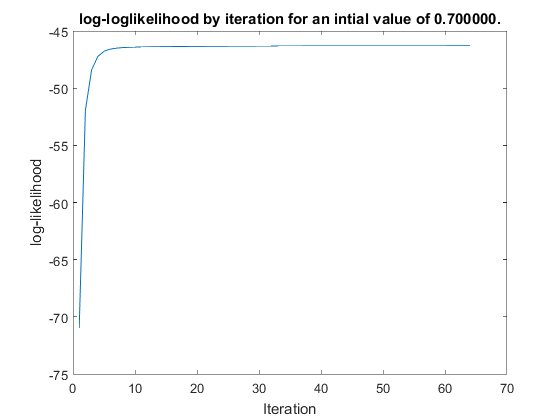
\includegraphics[width=0.7\linewidth]{images/LL7}
\label{fig:LL7}
\end{figure}
\textit{Graphs showing the log-likelihood against EM iteration number for initial values of 0.3 and 0.7, note the significantly larger number of iterations required to converge in the case of 0.3.}
\newpage
Overcoming the dependence on initial values can be achieved either by using standard methods of minimising the risk of finding local maxima, such as simulated annealing or more simply random restart hill climbing. Ueda et al. developed a deterministic annealing algorithm for EM.\cite{ueda1998deterministic} Alternatively, analysing the data to find clusters and choosing values based on this analysis has been explored, Karlis and Xekalaki\cite{karlis2003choosing} investigated several methods of \textit{'bootstrapping'} initial values using algorithms, for example by finding the means of the clusters in the data and using those as initial values.

\section{Task 3}
\subsection{Qualitative Description of the algorithms}
\subsubsection{Locally Linear Embedding}
LLE first generates a list of neighbours for each data-point on the manifold. Then, using the assumption that the neighbourhood lies on a locally linear plane, a barycentric coordinate for each data-point is constructed as a weighted linear combination of its neighbours. These weights are then used in the lower dimensional space to re-construct the data-point. As each locally linear neighbourhood is overlapping, it is possible to re-construct the entire dataset in the low dimensional space. An error function is used for both the weight generation and point re-construction phases, to produce an optimal solution.
\subsubsection{Laplacian eigenmaps}
This algorithm generates a weighted neighbourhood graph of the high dimensional data, with weights either being a 1 for each neighbour or generated using a heat kernel to better represent distance between points. The graph acts as a representation of the manifold in high dimensional space. The graphs laplacian matrix is then generated from the weight matrix and its diagonal. The solutions to the generalized eigenvector problem for this Laplacian matrix can be used as a function for the embedding, with dimensionality reduction achieved by removing eigenvalues starting from the smallest.
\subsubsection{Isomap}
Isomap can be thought of as an extension of Multi Dimensional Scaling, as it attempts to plot every data point in a lower dimensional space such that the high dimensional distances between data-points are maintained as best as possible. The distance metric is an estimate of geodesic distance between points over the manifold, generated by summing the euclidean distance between nodes on the shortest path between the nodes over a neighbourhood graph. Step 1 generates the neighbourhood graph, either with k-nearest neighbours or fixed radius, then the shortest paths between nodes are calculated and finally the estimated geodesic distance is used to apply MDS.
\subsection{Comparing the methods for embedding data into vector space}
When comparing the embeddings between vector spaces generated by the algorithms the main point of difference is the ability of ISOMAP to represent the global structure of the data more accurately than LLE and Laplacian Eigenmaps. As both LLE and LE are local techniques, the relationships between data points are only assured to be maintained over a local neighbourhood, with the global structure of the data potentially being warped or changed. On the other hand, ISOMAP ensures that the global structure of the data is conserved along with the local relationships, this is called having an isometric embedding. LLE has conformal embedding, as it replicates distances locally. Laplacian Eigenmaps have an embedding similar to conformal embedding, but this is dependant on the data.\cite{cayton2005algorithms} Therefore, on a global scale ISOMAP will produce a more truthful representation of the high dimensional data than LLE or LE. 

As ISOMAP preserves global structure via geodesic distances over the manifold it is much more susceptible to \textit{short circuit} errors, where the neighbourhood radius chosen is bigger than features in the manifold, such that points in the neighbourhood are on opposite sides of a gap in the manifold. This can also happen in LLE and Laplacian eigenmaps, but as the embeddings are local the problem is minimised. In ISOMAP, a single short circuited distance can have a knock on effect on many of the geodesic distances used for finding shortest paths over the graph. For this reason, ISOMAP is generally restricted to manifolds with intrinsically convex data and holes in the data will cause problems. Convex parameter space is not a requirement for the LLE and Laplacian Eigenmap algorithms.

A constraint on the usage of LLE and Laplacian eigenmaps is that the dimensionality of the high dimensional space must be known before the algorithms are run, as they are used in the algorithms to generate the embedding. This is not the case with ISOMAP and so it can be used in cases where this information is not available. 

Computational complexity is also a consideration when comparing the algorithms. ISOMAP is significantly more complex to calculate due to the geodesic distances being calculated and therefore can be problematic when applied to very large datasets. On the other-hand, LLE and laplacian eigenmaps can take advantage of sparse matrix computations when they are calculating eigen pairs and as such scale much better to large datasets. However, ISOMAP is the only algorithm with a guarantee of global optimality.

In datasets that have been non-uniformly sampled, then Laplacian Eigenmap will not necessarily converge to the Laplace-Beltrami operator\cite{belkin2007convergence}, therefore data uniformly sampled over a manifold is a requirement for Laplacian Eigenmaps, a requirement not needed for ISOMAP and LLE.
\subsection{Describing the methods mathematically}
\subsubsection{Locally Linear Embedding}
LLE begins by computing the neighbours for each data-point $x_i$ in $X = \{\vec{x}_1,...,\vec{x}_N\}$ either by placing a threshold on euclidean distance $\epsilon$, such that $x_j$ is a neighbour of $x_i$ if the euclidean distance in the high dimensional space $d_x(x_i,x_j) < \epsilon$. Alternatively, neighbours can be assigned based on $k$ nearest neighbours. We now need to compute the weights for each of the neighbours such that we can reconstruct the data-point as a linear combination of its neighbours. The following method is descried here.\cite{LLERoweis} First, we take the matrix $Z$, consisting of every neighbour of $x_i$ and subtract $x_i$ form every neighbour, we then compute the local co-variance of each element: $C = Z^TZ$. By solving $Cw = 1$ we find the weightings for each neighbour. We create an N by N matrix $W$ to store these weights, with $W_{ij}$ being 0 if $x_j$ is not a neighbour of $x_i$ and $\frac{w}{sum(w)}$ if they are neighbours.\\
We can now use this weight matrix to reconstruct $X$ in a lower dimensional space $d<<D$ with embedding $Y$. We do this by minimising the error function $\min_Y\sum\limits_{i}|Y_i-\sum\limits_{j}W_{ij}Y_j|^2$.\cite{ghodsi2006dimensionality} The embedding $Y = \{\vec{y}_1,...,\vec{y}_N\}$ is found finding the eigenpairs for the matrix $M = (I-W)^T(I-W)$ and setting the rows of $Y$ to the ascending eigenvectors after discarding the eigenvector with a corresponding eigenvalue of 0. $y_i = (f_1(_i),...,f_m(_i))$ with $f$ being an eigenvector solution to the above matrix.
All algorithms and formulas taken from \textit{'Nonlinear dimensionality reduction by locally linear embedding'}\cite{roweis2000nonlinear} except where cited.
\subsubsection{Laplacian Eigenmaps}
The Laplacian Eigenmaps algorithm again starts by computing the nearest neighbours for every vector in $X = \{\vec{x}_1,...,\vec{x}_N\}$, either by using k-nearest neighbours or euclidean distance. This is stored as a graph, with an edge between each pair of data points which are neighbours. A weight is added to each edge, either simply 1 for each connection, creating an adjacency graph or by using a heat kernel function $W_{ij}=e^{-\frac{||X_i-x_k||^2}{t}}$. As t increases, the W value gets closer to the simple approach.\cite{hagueeigen} \\
We then compute the eigenpairs for the generalised eigen problem: $Lf = \lambda Df$ where D is a diagonal matrix formed by summing each row of W: ($D_{ii} = \sum\limits_jW_{ji}$) $L$ is the Laplacian matrix, which is calculated by $L = D-W$. By ordering the solutions to this formula, f, by the size of the associated eigenvalue and by removing the first f, which corresponds to an eigenvalue of 0 we can map the $X$ values to $Y$ values in m-dimensional space: $y_i = (f_1(_i),...,f_m(_i))$
All algorithms and formulas taken from \textit{'Laplacian eigenmaps for dimensionality reduction and data representation'}\cite{belkin2003laplacian} except where cited.
\subsubsection{Isomap}
Starting with a set of $N$ data-points $X = \{\vec{x}_1,...,\vec{x}_N\}$ we first create a weighted graph, $G$, of the neighbourhood relations of X. For each data-point $x_i$ we calculate its neighbouring points $X_n = \{\vec{x}_1,...,\vec{x}_j\}$ either by placing a threshold on euclidean distance $\epsilon$, such that $x_j$ is a neighbour of $x_i$ if the euclidean distance in the high dimensional space $d_x(x_i,x_j) < \epsilon$ or alternatively, neighbours can be assigned based on $k$ nearest neighbours. An edge is then placed in $G$ between each data-point and its neighbours, with the edge weight being the euclidean distance between them. \\
Now we must generate a distance matrix $D_G$ of the geodesic distance between all points in $G$. We initialise this matrix by inserting the euclidean distance between points that are connected, $d_G(i,j) = d_x(i,j)$ if $i$ and $j$ are connected in the graph. If the points are not connected we need to estimate the geodesic distance between them by minimising the combined weights of the edges in the path between them over the graph. This is effectively finding the shortest path between every two points. In Isomap, this is achieved using the Floyd–Warshall algorithm.\cite{floyd1962algorithm} Thus $ d_G(i,j) = min\{d_G(i,j),d_G(i,k) + d_G(k,j)\}$ for all values of k. \\
Now that we have a pairwise geodesic distance matrix for $X$ we can apply the classic Multi Dimensional Scaling algorithm by calculating a kernel matrix, by double centring the distance matrix: $K = -\frac{1}{2}(I - \frac{J}{n})D_G(I-\frac{J}{n}))$ where J is an n-by-n matrix of 1's and I is the identity matrix. We then eigen decompose the kernel matrix $K = U\Lambda U^T$. After removing negative eigenvalues we then set $Y = \Lambda^{\frac{1}{2}}U^T$. The dimensionality of $Y$ is adjustable by removing eigenvalues and vectors from their respective matrices, in order of size.

All algorithms and formulas taken from \textit{'A Global Geometric Framework for Nonlinear Dimensionality Reduction'}\cite{tenenbaum2000global} except where cited.

\subsection{Description of a paper}
\textit {'Wireless sensor networks localization with isomap'} by Wang et al,\cite{wang2009wireless} was chosen by searching the articles citing the Isomap paper on Google Scholar, because of the novel use of Isomap in finding location estimates for wireless sensors using pairwise dissimilarity. The data can be represented on a graph as a neighbourhood graph with edge weights being radio signal strength data, also used as the euclidian distance for ISOMAP. As the data is error prone over long distances, Isomap is used as an extension of MDS, a strength of this implementation. Additionally, they developed a centralised system, where isomap is better suited due to its global algorithm, LLE is used in decentralised applications.\cite{patwari2004manifold} The primary problem they encountered was setting the number of neighbours to choose for step 1 of Isomap, they overcame this by using an adaptive parameter selection method.
\bibliography{report}{}
\bibliographystyle{IEEEtranN}
\end{document}